\begin{figure}[htbp]
\centering
\begin{tikzpicture}[x=1.9cm,y=1.05cm,>=Stealth,font=\small]
\foreach \j/\lab in {0/0,1/1,2/2,3/3,5/12}{
  \node[circle,fill=black,inner sep=1.6pt,label=above:{$a_{\lab}$}] (a\j) at (\j,1.4) {};
  \node[circle,fill=black,inner sep=1.6pt,label=below right:{$b_{\lab}$}] (b\j) at (\j,0) {};
  \node (q\j) at (\j,-1) {$q_{\lab}$};
  \draw[->] (b\j) -- (q\j);
}
\foreach \j/\prev in {1/0,2/1,3/2}{
 \draw[->] (a\prev)--(a\j);\draw[->] (b\prev)--(b\j);
 \draw[->,blue!65!black,thick] (a\j)--node[right]{$d_{\j}$}(b\j);
}
\draw[->,blue!65!black,thick] (a5)--node[right]{$d_{12}$}(b5);
\draw[dashed,->] (a3)--(a5);\draw[dashed,->] (b3)--(b5);
\node at (4,.7) {$\cdots$};
\node[left] at (a0) {$s_2$};\node[left] at (b0) {$s_1$};
\end{tikzpicture}
\caption{Réseau planaire à deux lignes. Les arêtes horizontales et de sortie ont un poids égal à un. Chaque chemin depuis la source supérieure descend une seule fois. Pour deux destinations \(i<j\), les paires disjointes descendent après \(i\) et avant \(j\) ; leur poids total est \(\Delta_{ij}=d_{i+1}+\cdots+d_j\). Les traits discontinus conservent les huit positions intermédiaires omises uniquement dans le dessin.}
\end{figure}

\begin{figure}[htbp]
\centering
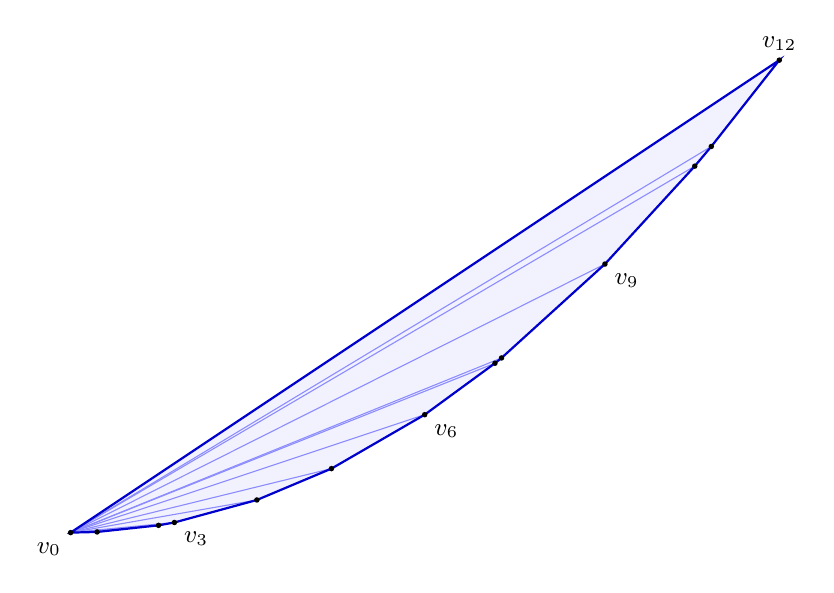
\begin{tikzpicture}[x=9cm,y=6cm,font=\small]
\foreach \j/\num in {0/0,1/234,2/777,3/917,4/1646,5/2305,6/3129,7/3750,8/3808,9/4722,10/5516,11/5662,12/6263}{
 \pgfmathsetmacro{\tx}{\num/6263}
 \coordinate (v\j) at (\tx,\tx*\tx);
}
\fill[blue!5] (v0)--(v1)--(v2)--(v3)--(v4)--(v5)--(v6)--(v7)--(v8)--(v9)--(v10)--(v11)--(v12)--cycle;
\foreach \j in {2,...,11}{\draw[blue!45,thin] (v0)--(v\j);}
\draw[blue!80!black,thick] (v0)--(v1)--(v2)--(v3)--(v4)--(v5)--(v6)--(v7)--(v8)--(v9)--(v10)--(v11)--(v12)--cycle;
\foreach \j in {0,...,12}{\fill (v\j) circle[radius=.035cm];}
\node[below left] at (v0) {$v_0$};
\node[below right] at (v3) {$v_3$};
\node[below right] at (v6) {$v_6$};
\node[below right] at (v9) {$v_9$};
\node[above] at (v12) {$v_{12}$};
\end{tikzpicture}
\caption{Polygone rationnel déterminé par les treize paramètres
\(t_j\) de \eqref{eq:polygon-Z}, dessiné avec ses coordonnées effectives
\((t_j,t_j^2)\). La triangulation à partir de \(v_0\) comporte onze cellules.
Chaque diagonale intérieure reçoit deux résidus opposés. Cinq
sommets sont étiquetés pour faciliter la lecture ; les treize sont représentés.}
\end{figure}
